
\chapter{Contribution and Results}
\minitoc
\thispagestyle{empty}
\newpage

\section{Introduction}
Nous présentons dans ce chapitre les notions vues dans les chapitres précédents appliquer à un dataset. Partant de la collecte et la préparation du dataset, de l’application de la théorie des réponses aux items pour un ajustement bayésiens des réponses obtenues par les apprenants, jusqu’aux clustering hard et soft des items basés sur la similarité.

\section{Approche proposée}


\section{Implémentations et résultats expérimentaux}

\subsection{Outils de développement}
les outils matériels et logiciels utilisés pour le développement sont :

\subsubsection{Materiels}

\begin{table}[H]
  \centering
  \begin{tabular}{cccc}
    \toprule
     \textbf{Marque} & \textbf{CPU} & \textbf{RAM} & \textbf{OS} \\
     \midrule
       \textbf{Lenovo Y40-80} & AMD Intel Core i5 2.20 GHz & 16Go & Windows10 64bits \\ \hline
       \multicolumn{4}{m{14cm}}{\centering Et Linux Ubuntu 20.04 LTS installé sur WSL2 }\\
    \bottomrule
  \end{tabular}
  \caption{Caractéristiques du matériels utilisés}
  \label{tabmat}
\end{table}

\textbf{WSL2 :} Windows Subsystem for Linux (WSL) est une couche de compatibilité permettant d'exécuter des exécutables binaires Linux de manière native sur Windows 10 et Windows Server 2019. WSL2 est une version améliorer de WSL1 qui introduit d'importants changements, notamment la présence d'un véritable noyau Linux \cite{craigloewen_msft} via un sous-ensemble de fonctionnalités Hyper-V. 

\subsubsection{Outils et packages}

\begin{table}[H]
	\centering
	\addtolength{\leftskip} {-4cm}
	\addtolength{\rightskip}{-4.5cm}
	\begin{tabular}{|m{5cm}|m{14cm}|}
	\hline
	\rowcolor{blueforest}
	\color{white} \textbf{Outils | Packages} & \color{white} \textbf{Description}  \\
	\hline\hline
	\multicolumn{2}{|m{19cm}|}{\centering Les outils et packages utilisés sur windows 10 : }\\ \hline
	\begin{center}
	    \begin{minipage}{.3\textwidth}
      
\includegraphics[width=\textwidth]{images/chapitre7/python.png}
    \end{minipage}
	\end{center}
	\centering \textbf{Python} \cite{10.5555/1593511} & Créé par le développeur Guido Van Rossum et publié pour la première fois en 1991. Il permet aux programmeurs d'utiliser différents styles de programmation pour créer des programmes simples ou complexes. Python est l'un des langages de programmation les plus populaires pour la science des données. C'est un langage de programmation de haut niveau, structuré, open source, interprété et dynamique. Il est multiparadigme, multi-plateforme et multi-usages. La syntaxe de Python aide les programmeurs à coder en moins d'étapes par rapport à d'autres langages comme JAVA ou C++, ce qui facilite le travail et le rend plus rapide, facile et amusant à faire. Il possède une bibliothèque standard complète et volumineuse dotée d'une gestion automatique de la mémoire et de fonctionnalités dynamiques \cite{python_cours}. Dans notre travail, nous avons utilisé Python 3.5 intégré à Anaconda. \\ \hline
  \begin{center}
	    \begin{minipage}{.3\textwidth}
      
\includegraphics[width=\textwidth]{images/chapitre7/anaconda.png}
    \end{minipage}
	\end{center}
	\centering \textbf{Anaconda} & Anaconda \cite{anaconda_citation} est une distribution libre et open source \cite{anaconda_website} des langages de programmation Python et R appliqué au développement d'applications dédiées à la science des données et à l'apprentissage automatique (traitement de données à grande échelle, analyse prédictive, calcul scientifique), qui vise à simplifier la gestion des paquets et de déploiement. Les versions de paquetages sont gérées par le système de gestion de paquets conda \cite{conda_website} et est adapté pour Windows, Linux et MacOS. Anaconda fournit interface graphique qui permet de lancer des applications, de gérer les librairies avec gestionnaire de paquets conda, et les environnements de développement. Plusieurs applications sont disponibles par défaut comme JupyterLab, Jupyter Notebook, QtConsole5, Spyder, Glue, Orange, RStudio, Visual Studio Code.  \\ \hline
  
  \begin{center}
    \begin{minipage}{.3\textwidth}
    
\includegraphics[width=\textwidth]{images/chapitre7/jupyter.png}
  \end{minipage}
  \end{center}
  \centering \textbf{Jupyter Notebook} \cite{Kluyver2016jupyter} & Jupyter Notebook est un environnement de programmation interactif basé sur le web utilisé pour programmer en python, R, Ruby, Julia ou encore Scala qui permet de réalisé des notebooks contenant à la fois du texte en markdown et du code en Julia, Python, R etc.  \\ \hline

  \begin{center}
    \begin{minipage}{.3\textwidth}
    
\includegraphics[width=\textwidth]{images/chapitre7/scikit_learn.png}
  \end{minipage}
  \end{center}
  \centering \textbf{Scikit-learn} \cite{pedregosa2011scikit} & Scikit-learn est une bibliothèque libre Python destinée à l'apprentissage automatique. Elle propose un ensemble d'outils efficace clé en main pour l’analyse et l’exploration de données. Cette bibliothèque prend en charge les algorithmes de classifications, de régression, du clustering, la réduction de dimensionnalité et de prétraitement des données pour l'extraction et la normalisation des caractéristiques.  \\ \hline

  \end{tabular}
	\caption{Indice de validité du clustering Hard}
	\label{tools}
\end{table}

\newpage

\begin{table}[H]
	\centering
	\addtolength{\leftskip} {-4cm}
	\addtolength{\rightskip}{-4.5cm}
	\begin{tabular}{|m{5cm}|m{14cm}|}
	\hline
	\rowcolor{blueforest}
	\color{white} \textbf{Outils | Packages} & \color{white} \textbf{Description}  \\
	\hline\hline
  %  >>>>>>>>>>>>>>
	\begin{center}
	    \begin{minipage}{.3\textwidth}
      
\includegraphics[width=\textwidth]{images/chapitre7/pandas.png}
    \end{minipage}
	\end{center}
  \centering \textbf{Pandas} \cite{mckinney2010data} & Pandas est une bibliothèque écrite en Python qui permet la manipulation et l'analyse des données. Elle propose en particulier des structures de données et des opérations de manipulation de tableaux numériques et de séries temporelles. Elle propose principalement comme structures de données les Series, DataFrames, Panels, Panels4D. Et aussi des fonctionnalités comme la manipuler des données aisément et efficacement avec des index pouvant être des chaines de caractères, des outils pour lire et écrire des données structurées, gestion des données manquantes, le tri, le redimensionnement et , fusion et jointure de large volume de données et analyse de séries temporelles. \\ \hline
  % <<<<<<<<<<<<<<

  %  >>>>>>>>>>>>>>
  \begin{center}
	    \begin{minipage}{.3\textwidth}
      
\includegraphics[width=\textwidth]{images/chapitre7/numpy.png}
    \end{minipage}
	\end{center}
	\centering \textbf{Numpy} \cite{2020NumPy-Array} & est une bibliothèque python pour le calcul scientifique qui fournit un objet tableau multidimensionnel, divers objets dérivés (tels que des tableaux et des matrices masqués) et un assortiment de routines pour des opérations rapides sur des tableaux, notamment mathématiques, logiques, manipulation de forme, tri, sélection, transformées de Fourier discrètes, algèbre linéaire de base, opérations statistiques de base, simulation aléatoire etc.  \\ \hline
  % <<<<<<<<<<<<<<
  \begin{center}
    \begin{minipage}{.3\textwidth}
    
\includegraphics[width=\textwidth]{images/chapitre7/matplotlib.png}
  \end{minipage}
  \end{center}
  \centering \textbf{Matplotlib} \cite{hunter2007matplotlib} & Matplotlib est une bibliothèque du langage de programmation Python destinée à tracer et visualiser des données sous formes de graphiques en 2 ou 3 dimensions \cite{tosi2009matplotlib}. Cette bibliothèque permet de produire divers tracés par exemple des histogrammes, des fonctions de Rosenbrock, spirale logarithmique, graphiques d'erreurs, nuages de points etc.  \\ \hline

  \end{tabular}
	\caption{Indice de validité du clustering Hard}
	\label{tools}
\end{table}

\newpage

\begin{table}[H]
	\centering
	\addtolength{\leftskip} {-4cm}
	\addtolength{\rightskip}{-4.5cm}
	\begin{tabular}{|m{5cm}|m{14cm}|}
	\hline
	\rowcolor{blueforest}
	\color{white} \textbf{Outils | Packages} & \color{white} \textbf{Description}  \\
	\hline\hline
	\multicolumn{2}{|m{19cm}|}{\centering Les outils et packages supplémentaires utilisés sur Linux Ubuntu 20.04 LTS installé sur WSL2 : }\\ \hline
	\begin{center}
	    \begin{minipage}{.3\textwidth}
      
\includegraphics[width=\textwidth]{images/chapitre7/stan.png}
    \end{minipage}
	\end{center}
	\centering \textbf{Stan} & Stan \cite{stan} est une plate-forme pour la modélisation statistique, l’analyse de données et la prédiction dans les sciences sociales, biologiques et physiques, l’ingénierie et les affaires. Il permet de spécifier les fonctions de densité de log afin d’obtenir une inférence statistique bayésienne complète avec échantillonnage MCMC (NUTS, HMC), une inférence bayésienne approximative avec inférence variationnelle (ADVI), une estimation du maximum de vraisemblance pénalisée avec optimisation (L-BFGS). La bibliothèque mathématique de Stan fournit des fonctions de probabilité différentiables et une algèbre linéaire (C++ autodiff). Stan peut être utilisé avec les langages d’analyse de données les plus populaires (R, Python, shell, MATLAB, Julia, Stata) et fonctionne sur toutes les principales plates-formes (Linux, Mac, Windows) \textbf{sauf la version 3 qui fonctionne sur Linux et Mac, c’est ce qui nous a poussée a utilisé Linux Ubuntu 20.04 LTS sur WSL2}. Dans l’implémentation nous avons utilisé Pystan 3.2.0 \cite{pystan} qui est une interface Python pour Stan, un package pour l'inférence bayésienne. \\ \hline
  \begin{center}
	    \begin{minipage}{.3\textwidth}
      
\includegraphics[width=\textwidth]{images/chapitre7/arviz2.png}
    \end{minipage}
	\end{center}
	\centering \textbf{ArviZ} & ArviZ \cite{arviz_2019} est un package Python pour l'analyse exploratoire des modèles bayésiens. Comprend des fonctions d'analyse postérieure, de stockage de données, de diagnostic d'échantillons, de vérification de modèle et de comparaison. Ce package de fournir des outils backend indépendants pour les diagnostics et les visualisations de l'inférence bayésienne en Python, en convertissant d'abord les données d'inférence en objets xarray \cite{arviz}.  \\ \hline
  
  \end{tabular}
	\caption{Indice de validité du clustering Hard}
	\label{tools}
\end{table}

\subsection{Collecte et préparation des données}
\label{collect_encoding}
\href{https://kdd.org/kdd-cup/view/kdd-cup-2010-student-performance-evaluation/Intro}{\color{blue}{KDD Cup 2010}} est une compétition d'exploration de données éducatives dans laquelle les participants sont chargés de prédire les performances des élèves aux problèmes algébriques en fonction des informations concernant les performances passées. \\
\textbf{Algèbre I 2005-2006} \cite{blog_kdd} est un jeu de données qui est fourni pour débuter et se familiarisé avec le format et le développement d’un modèle d’apprentissage. Une brève description du dataset initial avant l’étape du pre-processing est dans le tableau \ref{dataset_features_describe}.

\begin{table}[H]
	\centering
	\addtolength{\leftskip} {-4cm}
	\addtolength{\rightskip}{-4.5cm}
	\begin{tabular}{|m{5cm}|m{8cm}|m{4cm}|}
	\hline
	\rowcolor{blueforest}
	\color{white} \textbf{Caractéristique} & \color{white} \textbf{Description}  & \color{white} \textbf{Nombre Total}\\
	\hline
	\multicolumn{3}{|m{17cm}|}{\centering le nombre total de transactions = 809694. }\\ \hline
    \textbf{Anon Student Id} &  identifiant unique et anonyme d'un étudiant & 574 \\ \hline
    \textbf{Problem Name} &  identifiant unique d'un problème & 1084 \\ \hline 
    \textbf{Correct First Attempt} &  l'évaluation par le tuteur de la première tentative de l'étudiant 1 si correcte, 0 sinon. &  \\ \hline

    \multicolumn{3}{|m{17cm}|}{ \centering Et 11 autres carateristiques du dataset : \textbf{Row}, \textbf{Problem View}, \textbf{Step Start Time}, etc.} \\ \hline
  \end{tabular}
	\caption{Description et statistiques du jeu de données.}
	\label{dataset_features_describe}
\end{table}

\newpage
Les étapes suivies pour la collecte et la préparation du dataset sont illustré par la figure.

\begin{figure}[H]
	\begin{center}
		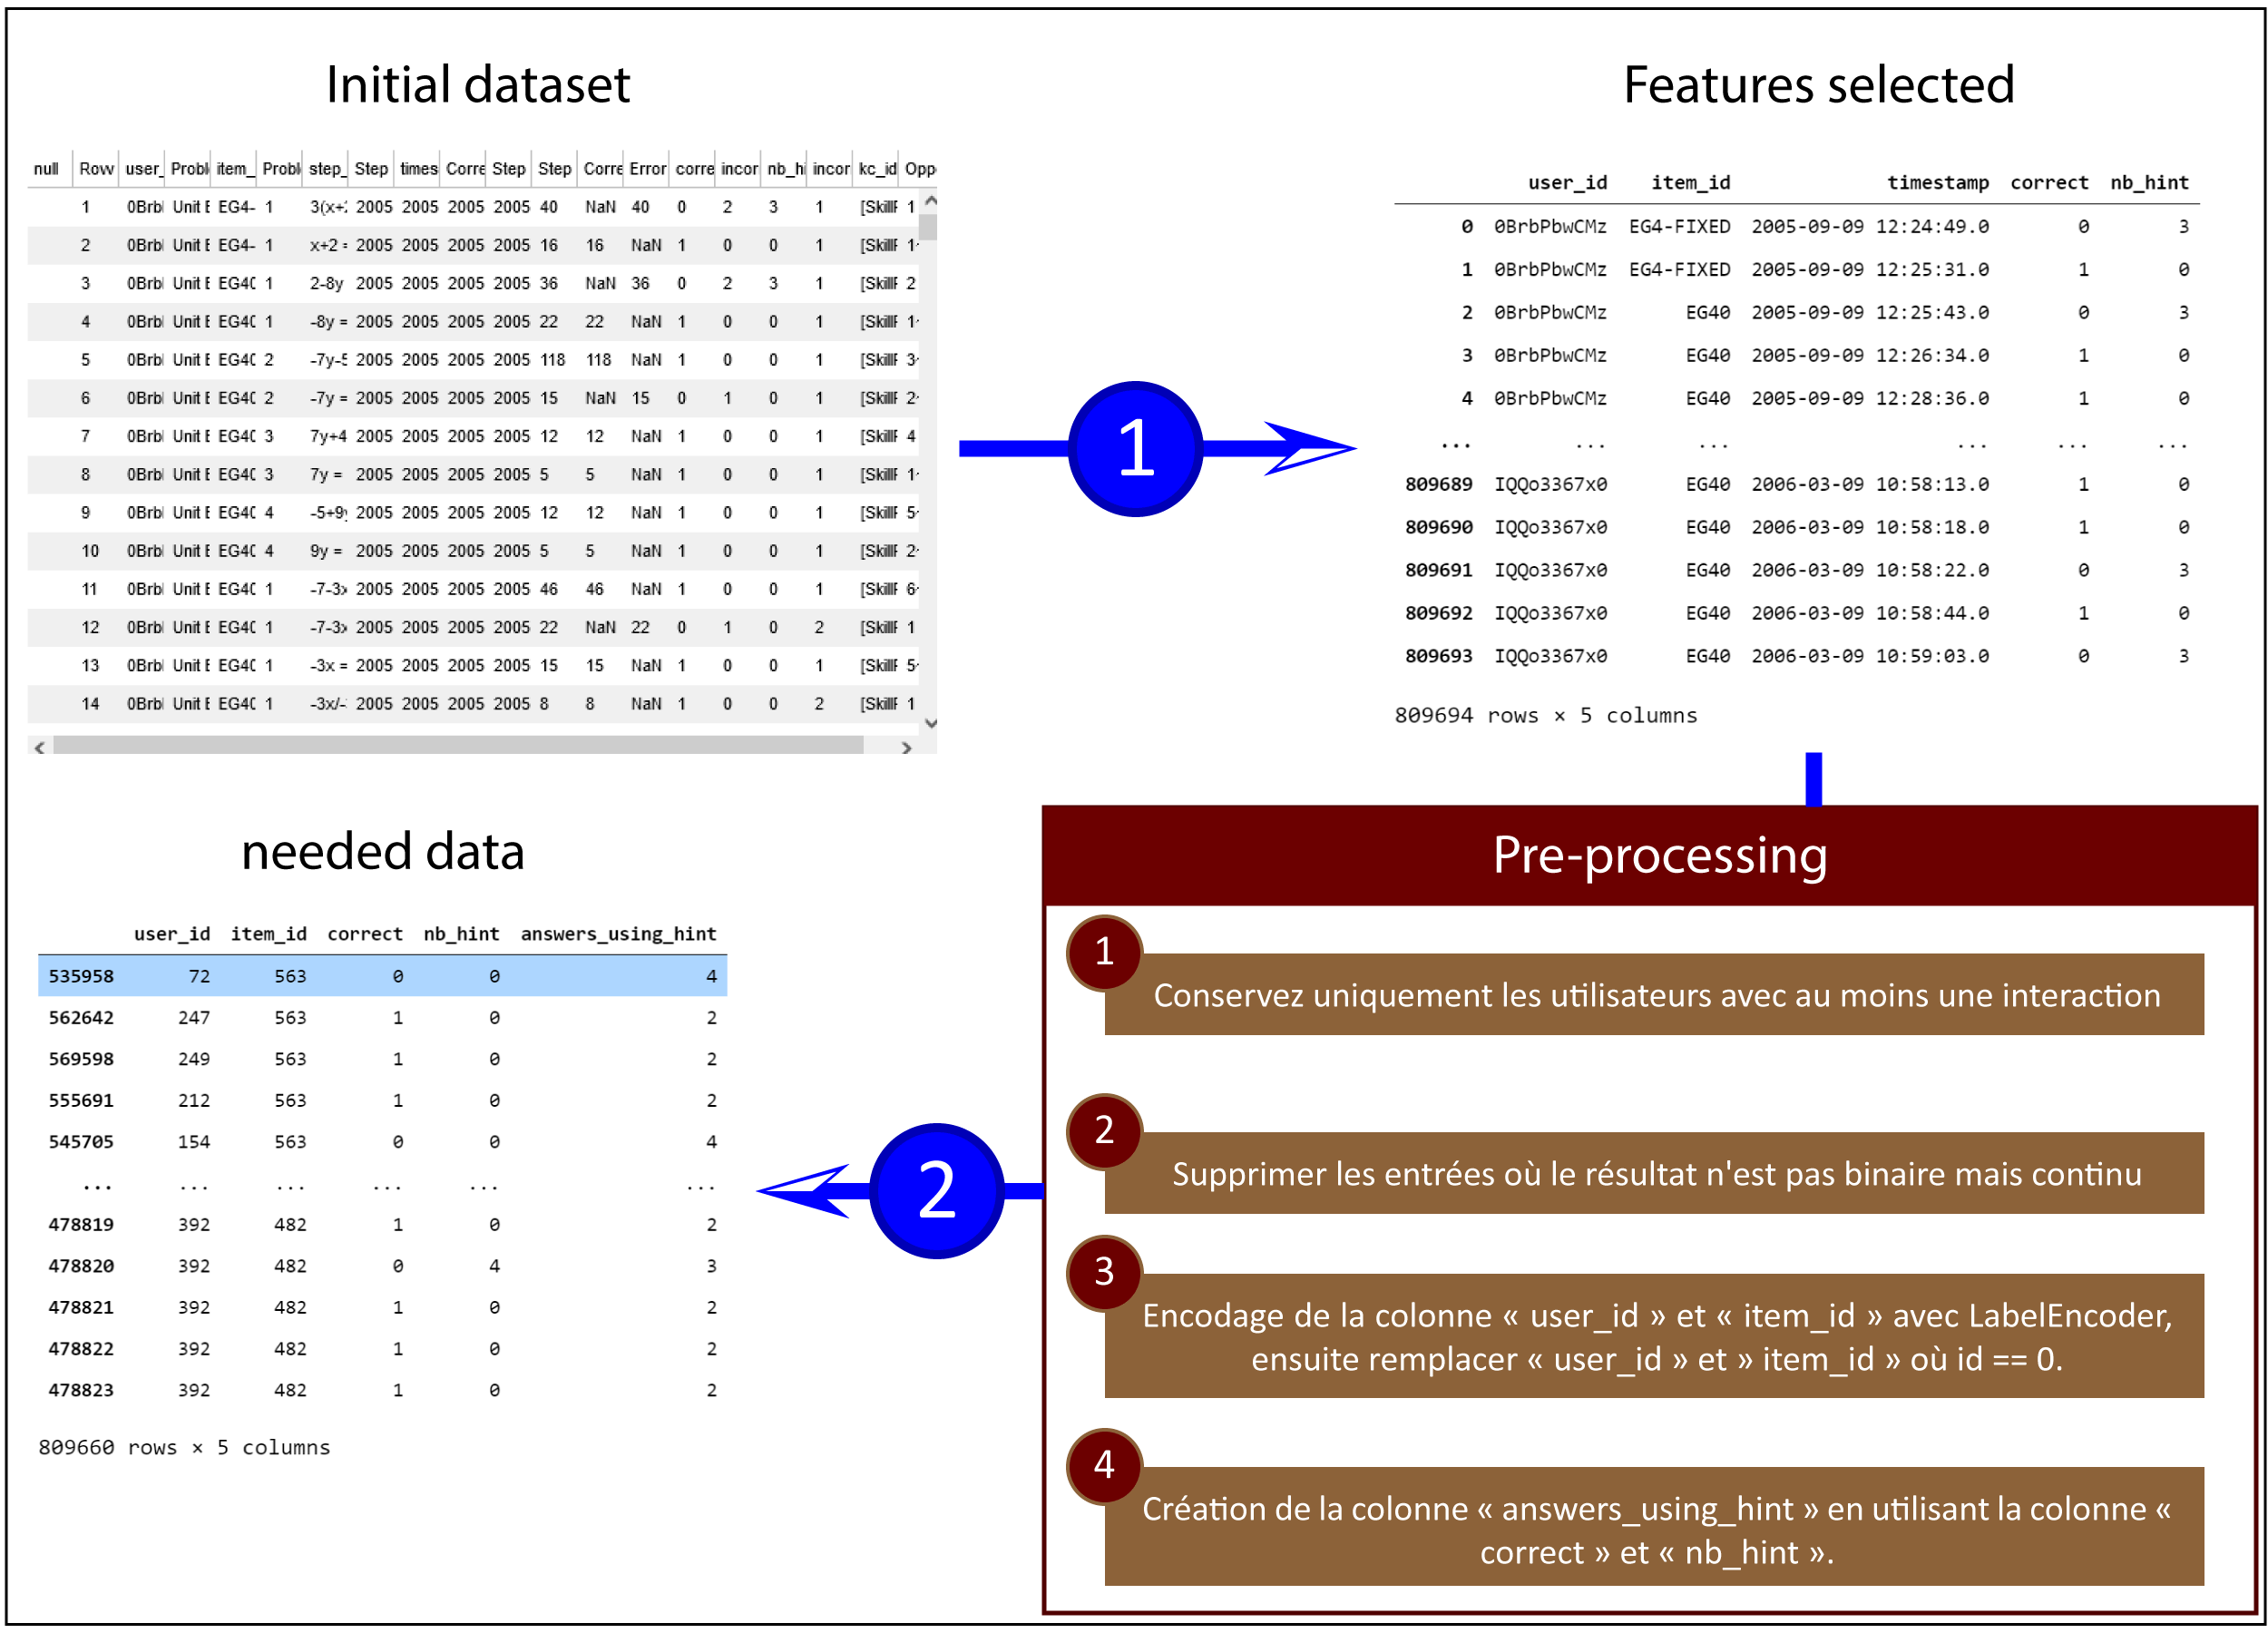
\includegraphics[width=\textwidth]{images/chapitre7/preprocessing_steps.png}
	\end{center}
	\caption{Le pre-processing du dataset.}
	\label{datatset_pre-processing}
\end{figure}

\begin{description}
    \item[\textbf{Première étape : }] dans notre travail, nous nous concentrons sur la performance de l'apprenant qui est liée à l'item, au résultat obtenu par l'apprenant : (correct/incorrect soit 0 ou 1), ou en prenant un indice (hint).
    \item[\textbf{Deuxième étape : }] seuls les apprenants ayant au moins 10 interactions avec les items ont été sélectionner. Les valeurs qui ne sont pas binaire (0 ou 1) dans la colonne « correct » sont éliminées. Les valeurs de la colonne « user\char`_id »  et « item\char`_id » sont encoder et où « id = 0 » est remplacer par le nombre total des apprenants et des items respectivement. L’encodage permet d’encoder les identifiants en valeur numérique, parce que le modèle IRT prend seulement des valeurs numériques à partir de 1. La colonne « answers\char`_using\char`_hint » ajouter au dataset sera utilisé pour calculer la matrice de similarité entre items selon notre critère : réponse correcte avec aide (hints) et sans aide, et incorrecte avec aide et sans aide.Le script python avec lequel la colonne « answers\char`_using\char`_hint » est dans \ref{answersusinghint}.
\end{description}

\newpage
\begin{lstlisting}[language=Python,label={answersusinghint}, 
	morekeywords={self},
	keywordstyle=\ttb\color{deepblue},
	emph={MyClass,__init__},
	emphstyle=\ttb\color{deepred},
	stringstyle=\color{deepgreen},basicstyle=\scriptsize, frame=l,framesep=4.5mm,framexleftmargin=2.5mm,tabsize=2,numbers=left,fillcolor=\color{blueforest!70},rulecolor=\color{blueforest},numberstyle=\normalfont\tiny\color{white}]
	conditions = [
		(needed['correct'] == 1) & (needed['nb_hint'] > 0),
		(needed['correct'] == 1) & (needed['nb_hint'] == 0),
		(needed['correct'] == 0) & (needed['nb_hint'] > 0),
		(needed['correct'] == 0) & (needed['nb_hint'] == 0)
		]
	# 1 ==> Correct avec hint
	# 2 ==> Correct sans hint
	# 3 ==> Incorrect avec hint
	# 4 ==> Incorrect sans hint
	values = [1, 2, 3, 4]
	
	# create a new column and use np.select to assign values to it using our lists as arguments
	needed['answers_using_hint'] = np.select(conditions, values)
\end{lstlisting}

\subsection{Modèle IRT pour une inférence bayésienne}

\subsubsection{Spécification et chargement du modèle}
Nous avons utilisé le modèle de Rasch pour faire l’ajustement bayésien avec Stan en utilisant le script en Stan définit dans le chapitre \ref{chap:irt}. Le script complet est :
\begin{lstlisting}[language=Stan,basicstyle=\scriptsize, frame=l,framesep=4.5mm,framexleftmargin=2.5mm,tabsize=2,numbers=left,fillcolor=\color{blueforest!70},rulecolor=\color{blueforest},numberstyle=\normalfont\tiny\color{white}]
_1pl_model = """
data {
	// numbers of things
	int<lower=1> N;  // number of observations
	int<lower=1> I;  // items,  number of questions  
	int<lower=1> S;  // subjects,  number of users 
	// data
	int<lower=1,upper=I> item[N];
	int<lower=1,upper=S> subject[N];
	int<lower=0,upper=1> grade[N];
}
parameters {
	// parameters
	real ability[S];             //  alpha: ability of student
	real difficulty[I];          //  beta: difficulty of question
	real delta;                   // mean student ability
}
model {
	ability ~ std_normal();         
	difficulty ~ std_normal();   
	delta ~ normal(0.75,1);
	for(n in 1:N)
		grade[n] ~ bernoulli_logit(ability[subject[n]] - difficulty[item[n]] + delta);
}
"""
\end{lstlisting}
Nous n’avons pas utilisé le bloc « generated quantities » parce qu’en ajoutant ce bloc la taille de modèle ajusté devient déraisonnablement grande. Avant de charger et compiler le modèle, Stan prend les données dans un dictionnaire, où les noms des clés doivent être identiques aux noms spécifiés dans la section data du modèle. Les données de notre dataset dans format dictionnaire est :

\begin{lstlisting}[language=Python,basicstyle=\scriptsize, frame=l,framesep=4.5mm,framexleftmargin=2.5mm,tabsize=2,numbers=left,fillcolor=\color{blueforest!70},rulecolor=\color{blueforest},numberstyle=\normalfont\tiny\color{white}]
	{'I': 1084,
	'N': 809660,
	'S': 569,
	'grade': array([0, 1, 1, ..., 1, 1, 1]),
	'item': array([563, 563, 563, ..., 482, 482, 482]),
	'subject': array([ 72, 247, 249, ..., 392, 392, 392])}
\end{lstlisting}

\subsubsection{Compilation du modèle et échantillonnage }

Après avoir spécifier le modèle, la compilation (en code c++) est faite en utilisant la fonction \colorbox{gray!30}{stan.build()} qui prend en paramètre le modèle , les données et random\char`_seed qui contrôle l’effet aléatoire. Le script est :
\begin{lstlisting}[language=Stan,basicstyle=\normalsize, frame=l,framesep=4.5mm,framexleftmargin=2.5mm,tabsize=2,numbers=left,fillcolor=\color{blueforest!70},rulecolor=\color{blueforest},numberstyle=\normalsize\tiny\color{white}]
	posteriori = stan.build(_1pl_model,data=train_data,random_seed=2021)
\end{lstlisting}

Une fois le modèle compiler avec les données, la méthode \colorbox{gray!30}{sample()} fait des échantillonnages dans les distributions spécifier dans le modèle. La méthode \colorbox{gray!30}{sample()} prend en paramètre \colorbox{gray!30}{num\char`_chains}   le nombre de chaine  qui sont exécuter en parallèle, \colorbox{gray!30}{num\char`_samples}  le nombre d’échantillon à générer, \colorbox{gray!30}{num\char`_warmup}  le nombre d’échantillon initial à rejeter qui sont généralement loin d'être optimales et \colorbox{gray!30}{num\char`_thin} spécifie un intervalle d'échantillonnage auquel les échantillons sont conservés.

\begin{lstlisting}[language=Stan,basicstyle=\normalsize, frame=l,framesep=4.5mm,framexleftmargin=2.5mm,tabsize=2,numbers=left,fillcolor=\color{blueforest!70},rulecolor=\color{blueforest},numberstyle=\normalsize\tiny\color{white}]
	fit = posteriori.sample(num_chains=2, num_samples=50000,
	      num_warmup=1000,num_thin=1)
\end{lstlisting}



\subsubsection{Résultats d’échantillonnage, diagnostique du modèle, prédiction et validation}


Une fois l’échantillonnage terminé, l’objet \colorbox{gray!30}{stanfit} renvoyer par la méthode \colorbox{gray!30}{sample()} contient la sortie dérivée de l’ajustement du modèle c’est-à dire les résultats de l’inférence. L’objet \colorbox{gray!30}{fit} du modèle est afficher dans le tableau de la figure \ref{stanfit_object}. La figure \ref{model_trace-plot} affiche les distributions postérieures des paramètres du modèle pour toute les itérations et la figure \ref{params_posterior_distribution} la moyenne des distributions postérieures.
\begin{figure}[H]
	\begin{center}
		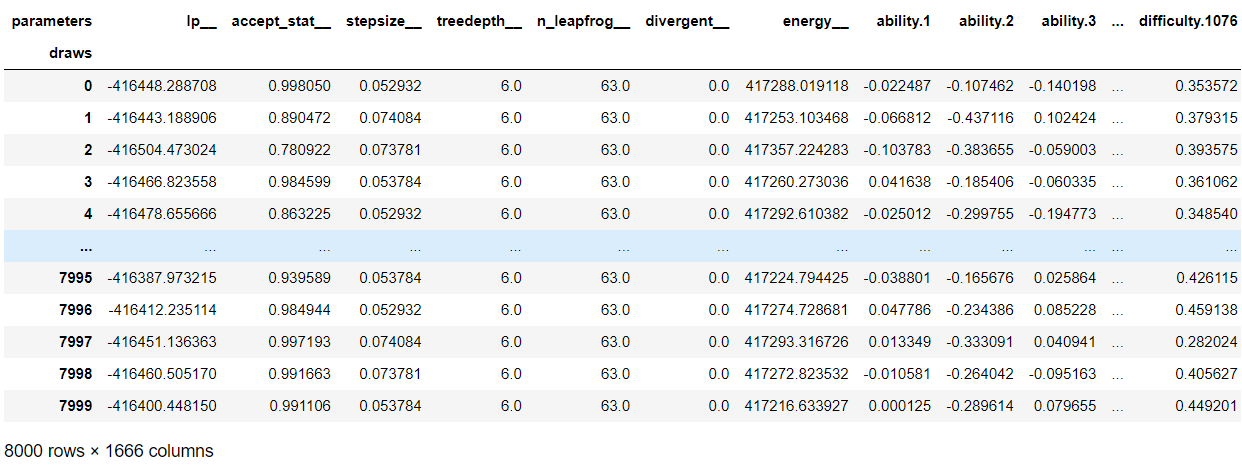
\includegraphics[width=\textwidth]{images/chapitre7/stanfit_object.png}
	\end{center}
	\caption{L’objet stanfit de notre modèle.}
	\label{stanfit_object}
\end{figure}


\begin{figure}[H]
	\begin{center}
		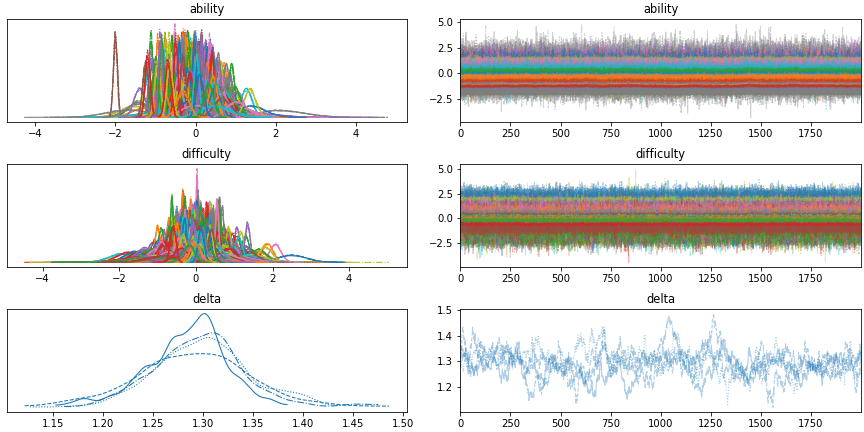
\includegraphics[width=\textwidth]{images/chapitre7/model_plot-trace.png}
	\end{center}
	\caption{Les distributions postérieures du modèle.}
	\label{model_trace-plot}
\end{figure}

\begin{figure}[H]
	\begin{center}
		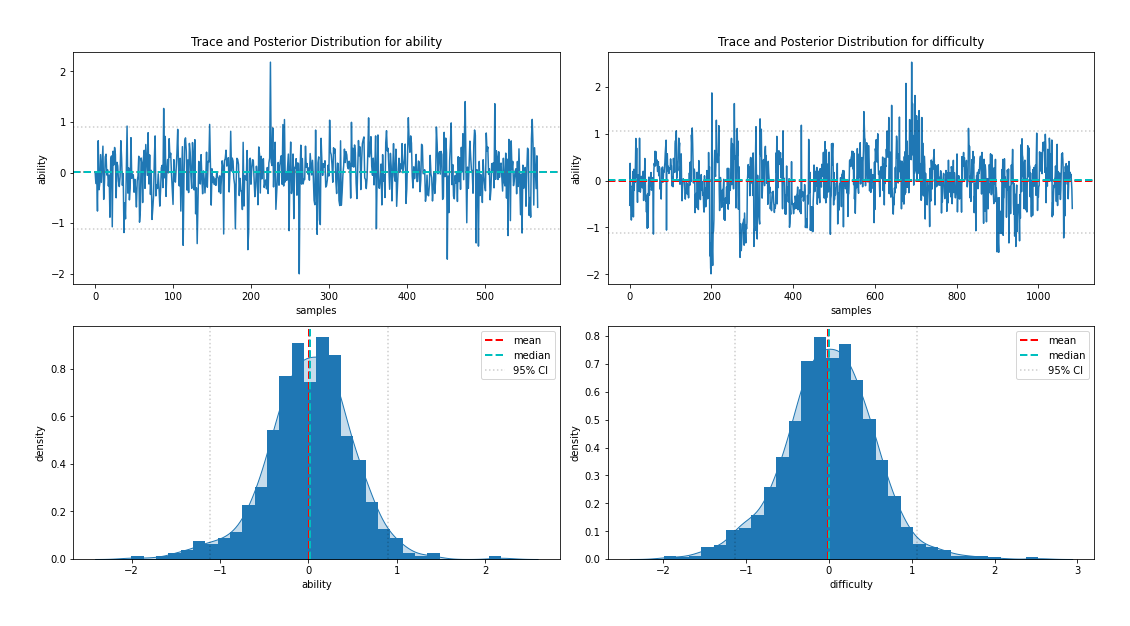
\includegraphics[width=\textwidth]{images/chapitre7/params_posterior_distribution.png}
	\end{center}
	\caption{La moyenne des distributions postérieures du modèle.}
	\label{params_posterior_distribution}
\end{figure}

En plus des valeurs des paramètres du modèle, le tableau de la figure contient également d’autre valeurs des paramètres utilisés par l'échantillonneur qui vont servir de diagnostique.
L'étiquette \colorbox{gray!30}{lp\char`_\char`_} est pour les densités logarithmiques (jusqu'à une constante additive), \colorbox{gray!30}{accept\char`_stat\char`_\char`_} est pour les probabilités d'acceptation, \colorbox{gray!30}{stepsize\char`_\char`_} est pour la taille de pas de l'intégrateur leapfrog pour simuler l'hamiltonien, \colorbox{gray!30}{treedepth\char`_\char`_} est la profondeur de l'arbre exploré par l'échantillonneur sans demi-tour (Journal base 2 du nombre d'évaluations de densité et de gradient log), \colorbox{gray!30}{n\char`_leapfrog\char`_\char`_} est le nombre d'évaluations de densité et de gradient, \colorbox{gray!30}{divergent\char`_\char`_} est un indicateur indiquant une instabilité numérique lors de l'intégration numérique entraînant la non conservation de l'hamiltonien, et \colorbox{gray!30}{energy\char`_\char`_} est la valeur hamiltonienne. \\

\textbf{Le BFMI :} Bayesian Fraction of Missing Information, bfmi inférieur à 0,2 indique qu’il faut peut-être reparamétrer votre modèle.

\begin{figure}[H]
	\begin{center}
		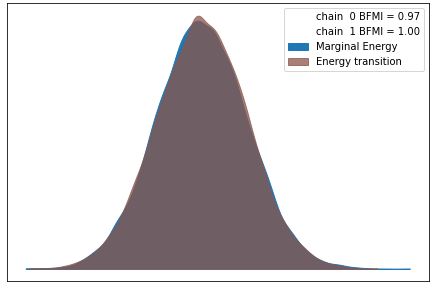
\includegraphics[scale=0.5]{images/chapitre7/model_energy.png}
	\end{center}
	\caption{BFMI du modèle.}
	\label{bfmi_of_model}
\end{figure}

\textbf{Le Rhat :} un Rhat > 1.1 indique généralement des problèmes d'ajustement et si Rhat est d'environ 1, alors il n’y aura aucune diminution de la variance d'échantillonnage, quelle que soit la durée d’itération, et donc la chaîne de Markov est susceptible (mais pas garantie) d'avoir convergé. Celui ne notre modèle est d'environ 1 pour tous les paramètres.

\begin{figure}[H]
	\begin{center}
		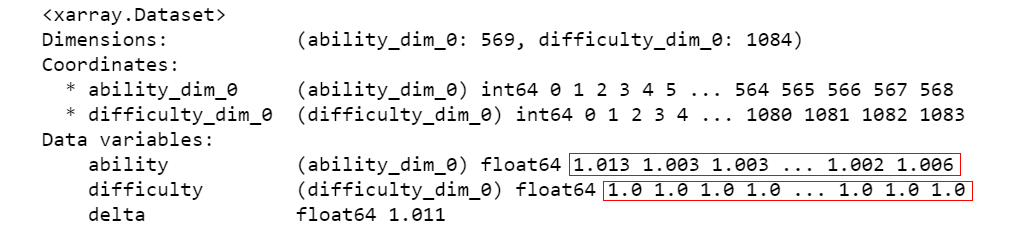
\includegraphics[width=\textwidth]{images/chapitre7/output_of_rhat.png}
	\end{center}
	\caption{Le Rhat du modèle.}
	\label{output_of_rhat}
\end{figure}
\textbf{Vérification des divergences }: aucune divergence dans le modèle comme le montre la figure \ref{diverging_output}.

\begin{figure}[H]
	\begin{center}
		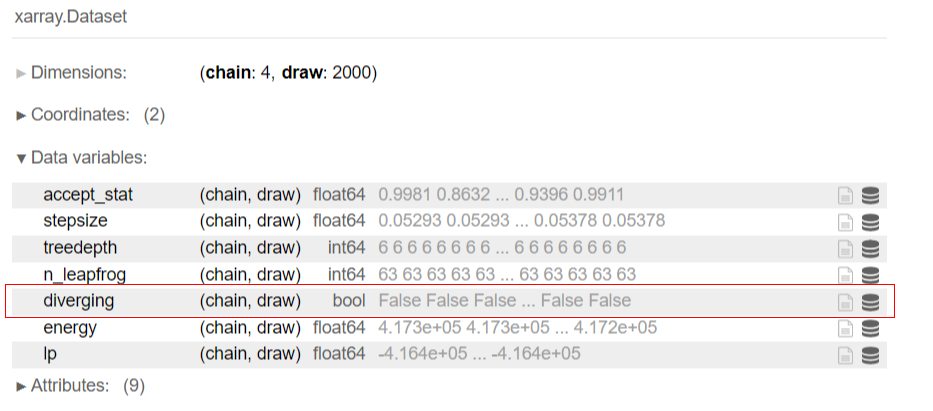
\includegraphics[width=\textwidth]{images/chapitre7/diverging_output.png}
	\end{center}
	\caption{La sortie de la divergence du modèle.}
	\label{diverging_output}
\end{figure}

Ensuite après diagnostique du modèle, les valeurs des paramètres obtenu peuvent être utilisé pour faire des prédictions postérieures en utilisant la fonction logistique de Rasch \ref{posterior_probability_distribution} ou bien faire des prédictions directement en utilisant le bloc generated quantities \ref{generated_quantities} et aussi récupérer le log de vraisemblance (log likelihood) qui est utilisé pour comparer plusieurs modèles (sélection de modèle). Mais l’utilisation de ce bloc entraine un coût de calcul et d'utilisation de la mémoire. Le script est utilisé pour prédire la probabilité de réussite à un item \ref{pred_script}. C’est ainsi que l’ajustement bayésien des réponses aux items a été fait avec un modèle d’inférence bayésien.

\begin{lstlisting}[language=Python,label={pred_script},stringstyle=\color{deepgreen},basicstyle=\scriptsize, frame=l,framesep=4.5mm,framexleftmargin=2.5mm,tabsize=2,numbers=left,fillcolor=\color{blueforest!70},rulecolor=\color{blueforest},numberstyle=\normalfont\tiny\color{white}]
ability = np.mean(fit['ability'],axis=1)
difficulty = np.mean(fit['difficulty'],axis=1)
y_pred = []
for i in range(0,len(needed)):
	diff = train_data['item'][i] # Item index
	abilt = train_data['subject'][i] # Subject index
	p = np.exp(ability[abilt - 1 ] - difficulty[diff - 1])/(1+np.exp(ability[abilt - 1] 
	   - difficulty[diff - 1]))
	y_pred.append(p)
y_pred = np.round(y_pred).astype(int)
\end{lstlisting}

Nous terminons donc cette étape avec la validation des prédictions faite par le script. Plusieurs métriques peuvent être utilisé pour valider les prédictions d’un modèle de classification parce qu’on a deux classes (réponses correcte ou incorrecte).

\begin{itemize}
	\item \textbf{Accuracy :}
	\item \textbf{Mean squared error :}
	\item \textbf{Roc auc score :}
	\item \textbf{Cohen kappa :}	
\end{itemize}
Celui du modèle sont afficher dans le tableau et roc\char`_auc\char`_score est illustré par la figure.

\begin{minipage}{\textwidth}
	\begin{minipage}[b]{0.49\textwidth}
	\centering
	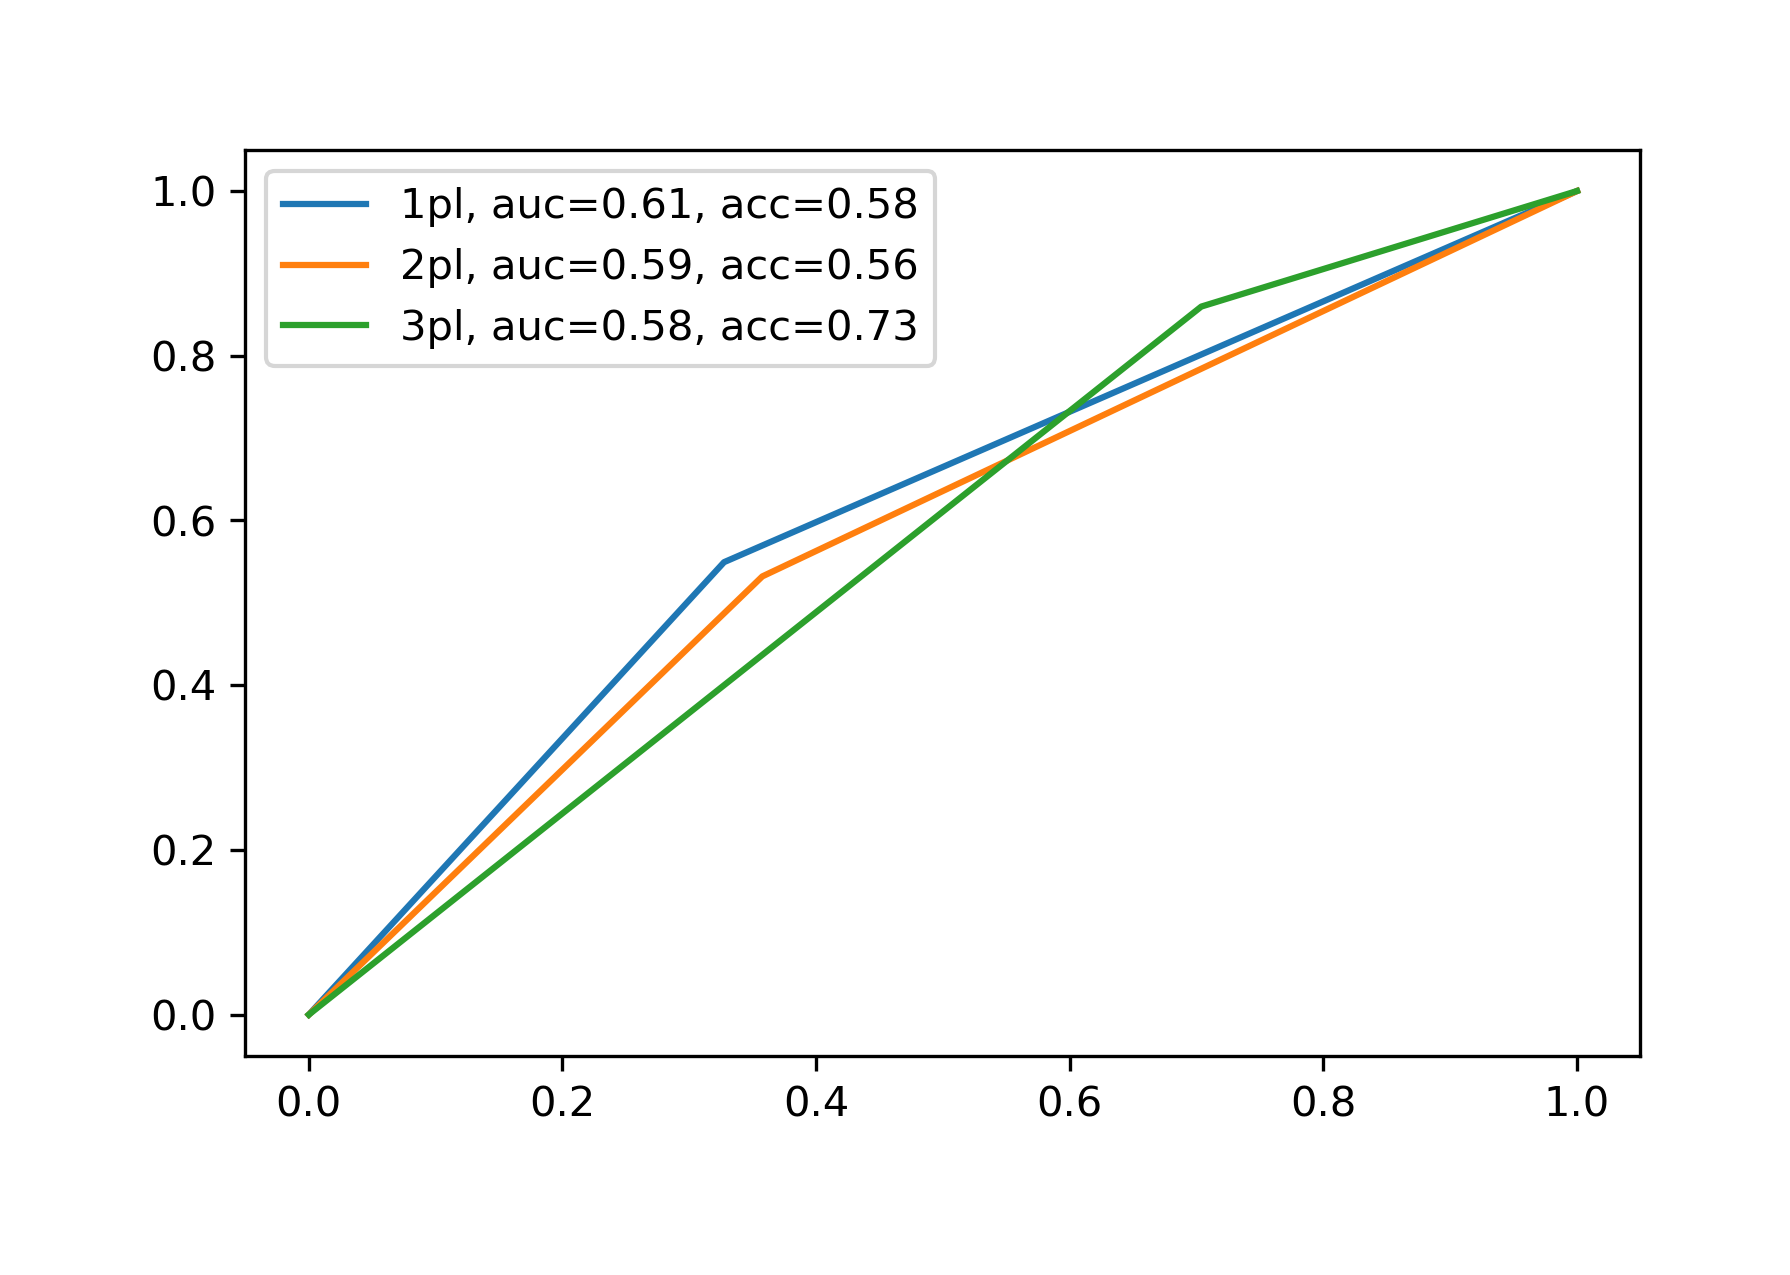
\includegraphics[width=\textwidth]{images/chapitre7/roc_auc.png}
	\captionof{figure}{A table beside a figure}
\end{minipage}
\hfill
\begin{minipage}[b]{0.49\textwidth}
	\centering
	\begin{tabular}{|m{3cm}|m{3cm}|}
	\hline
	\rowcolor{blueforest}
	\color{white} \textbf{Métriques} & \color{white} \textbf{valeurs}  \\
	\hline\hline
	mse & 0.421189 \\ \hline
	kappa & 0.1587 \\ \hline
	auc & 0.611 \\ \hline
	acc & 0.57881 \\ \hline
	\end{tabular}
	\captionof{table}{A table beside a figure}
	\end{minipage}
\end{minipage}

\subsection{Clustering hard et soft de la matrice de similarité}

\subsubsection{Création de la matrice de similarité}
Les données collecter dans la partie [\ref{collect_encoding}] et ceux de l’ajustement bayésien avec le modèle de Rasch (c’est-à dire les prédictions faites faire le modèle d’inférence bayésien) sont utilisée pour créer la matrice de réponse selon quatre catégories : correct avec aide (CH) et sans aide (CS), et incorrect avec aide (IH) et sans aide (IS). La matrice de réponses est ensuite utilisée pour créer la matrice de similarité entre items avec le coefficient de kappa. La figure \ref{similarity_steps} illustre toutes les étapes. 

\begin{figure}[H]
	\begin{center}
		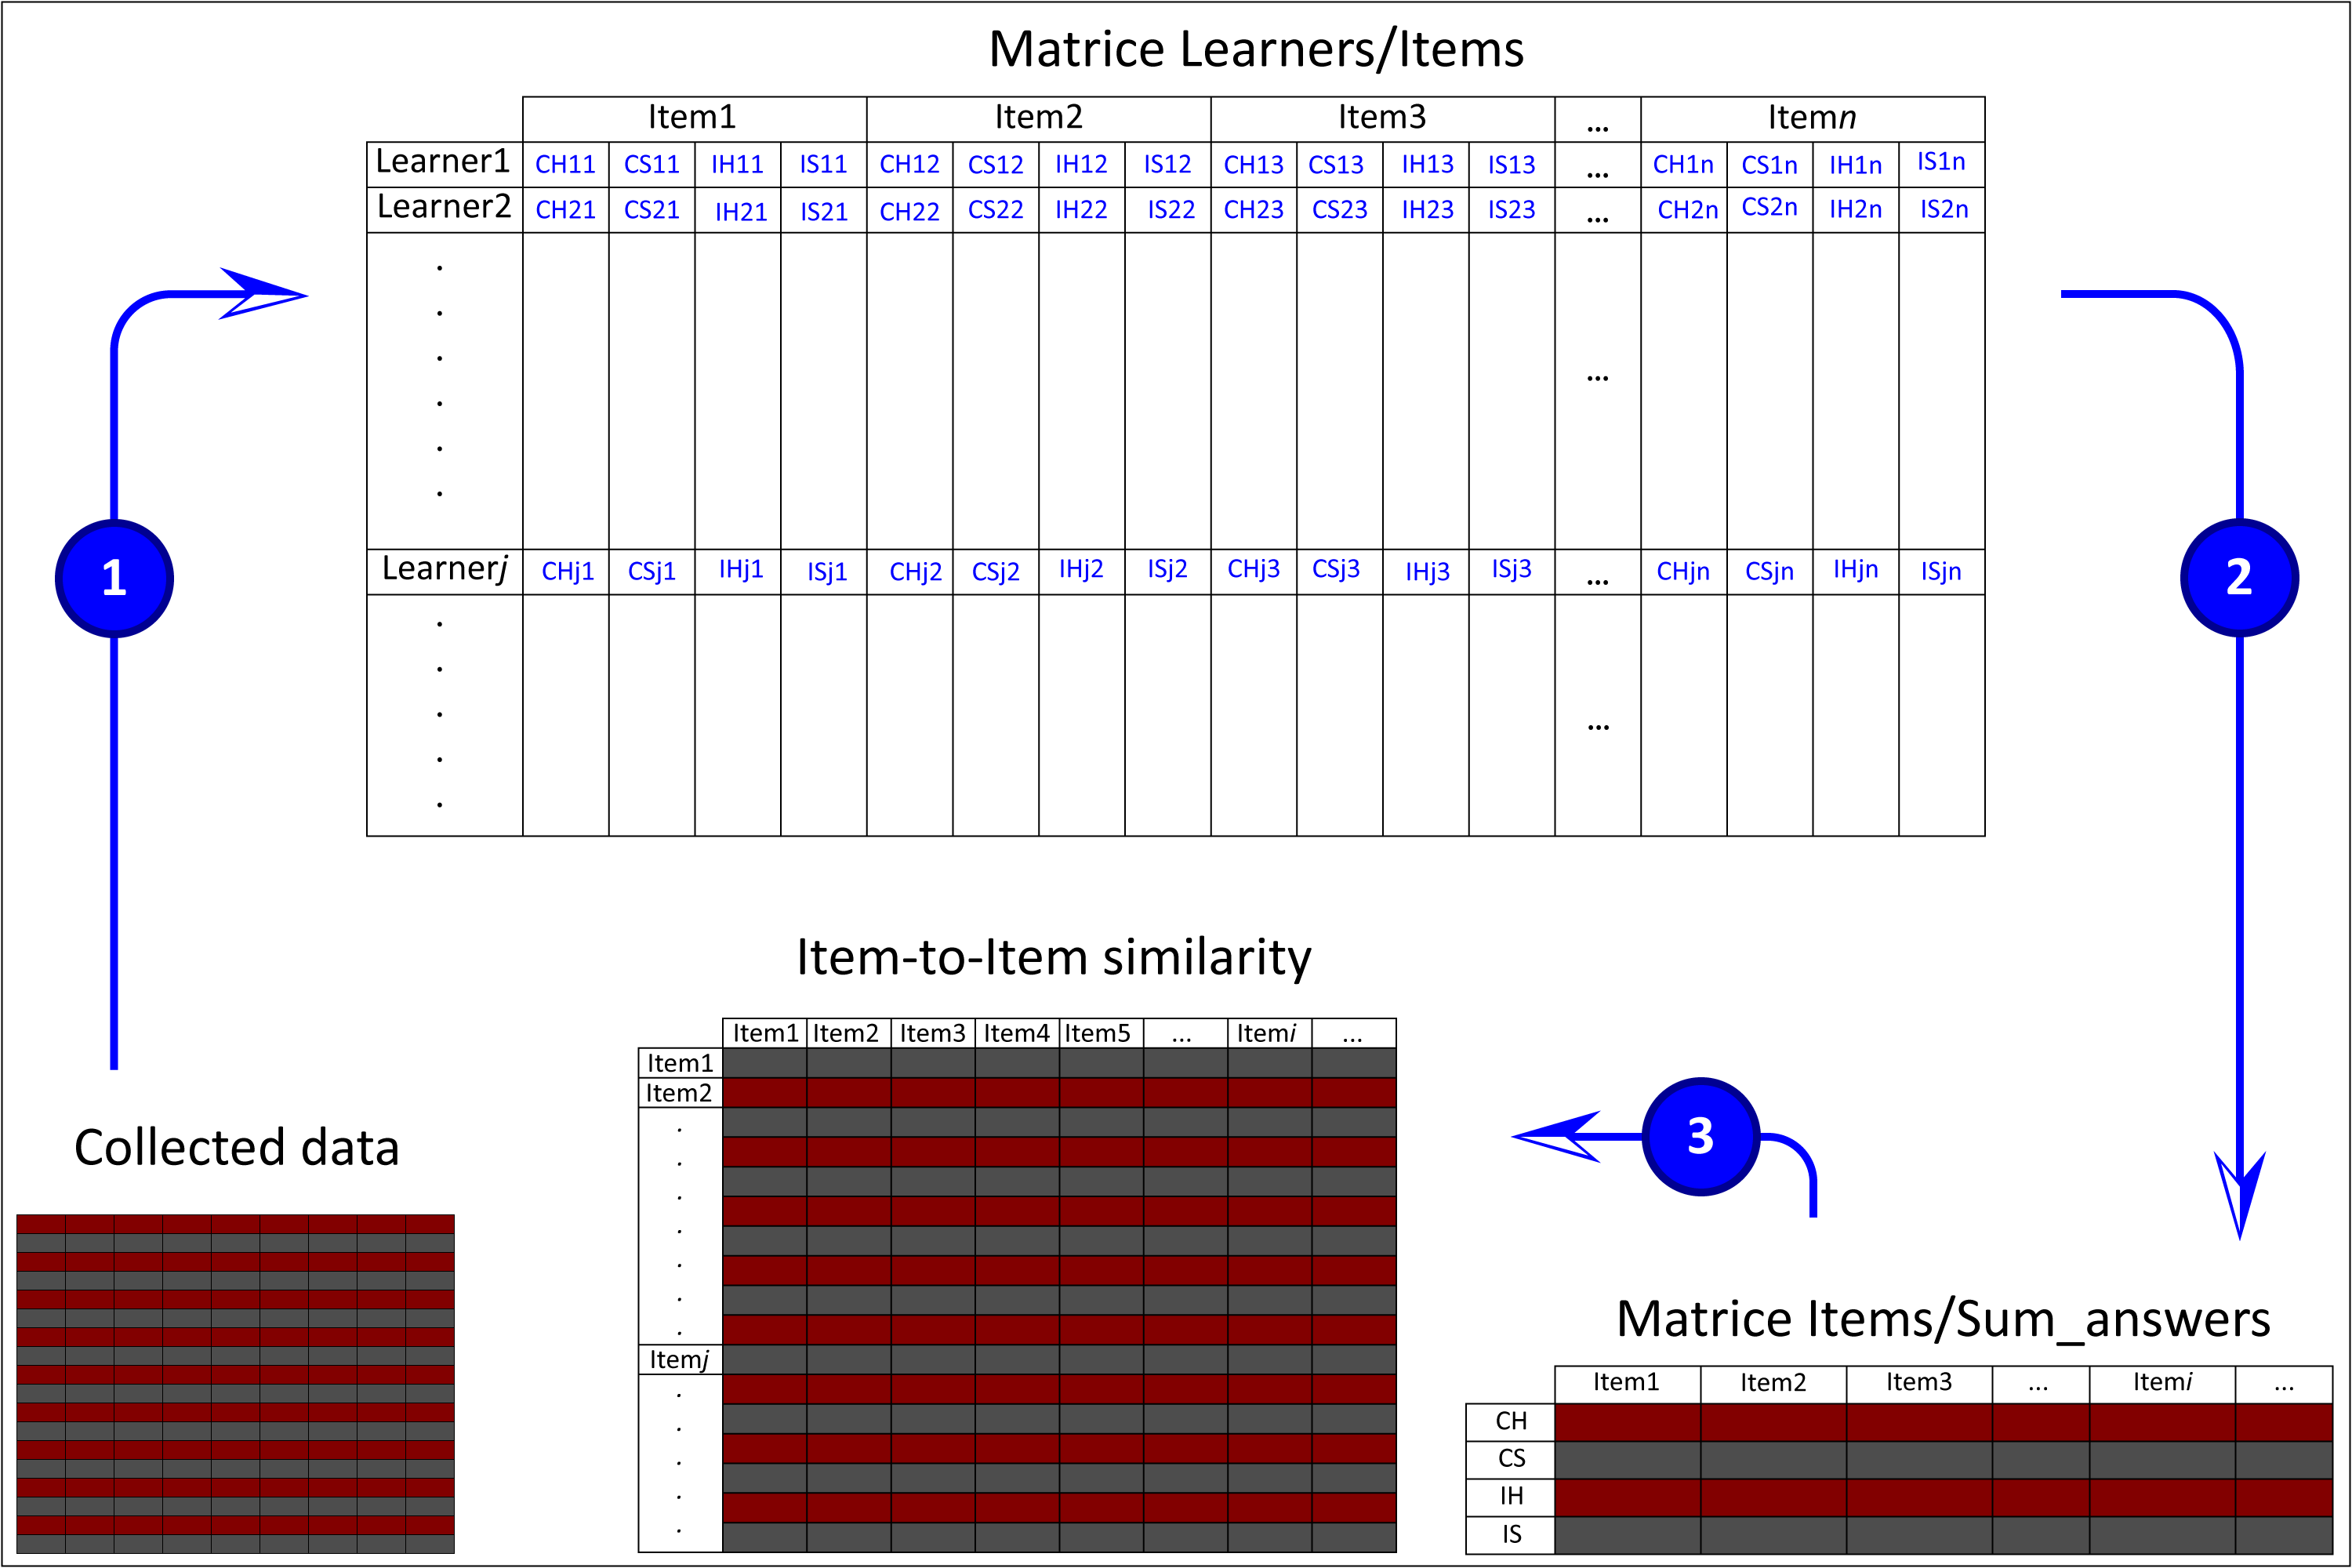
\includegraphics[width=\textwidth]{images/chapitre7/similarity_steps.png}
	\end{center}
	\caption{Les étapes de calcule de la matrice de similarité.}
	\label{similarity_steps}
\end{figure}

Le script utiliser pour calculer la matrice des sommes des réponses est :
\begin{lstlisting}[language=Python,basicstyle=\scriptsize, frame=l,framesep=4.5mm,framexleftmargin=2.5mm,tabsize=2,numbers=left,fillcolor=\color{blueforest!70},rulecolor=\color{blueforest},numberstyle=\normalfont\tiny\color{white}]
	def createSumMatrix(data):
    column_names = data['item_id'].unique()
    rows_name = ["CH","CS","IH","IS"]
    columns = pd.DataFrame(columns = column_names)
    index = pd.DataFrame(rows_name, columns = ['catégories'])
    sumOfAnswers_df = pd.concat([index,columns], axis=1)
    sumOfAnswers_df = sumOfAnswers_df.set_index("catégories")
    sumOfAnswers_df = sumOfAnswers_df.replace(np.nan,0)
    column_name = data['item_id'].unique()
    rows_name = data['user_id'].unique()
    for i in tqdm(rows_name):
        for j in column_name:
            dictVal = data[(data["user_id"] == i) & (data["item_id"] == j)]['answers_using_hint'].value_counts()
            chVal = sumOfAnswers_df.loc["CH",j]
            csVal = sumOfAnswers_df.loc["CS",j]
            ihVal = sumOfAnswers_df.loc["IH",j]
            isVal = sumOfAnswers_df.loc["IS",j]
            if len(dictVal) != 0:
                for key, value in dictVal.items():
                    key = int(key)
                    if key == 1:
                        chVal = int(chVal) + value
                    elif key == 2:
                        csVal = int(csVal) + value
                    elif key == 3:
                        ihVal = int(ihVal) + value
                    elif key == 4:
                        isVal = int(isVal) + value
                sumOfAnswers_df.loc["CH",j] = chVal
                sumOfAnswers_df.loc["CS",j] = csVal
                sumOfAnswers_df.loc["IH",j] = ihVal
                sumOfAnswers_df.loc["IS",j] = isVal
	return sumOfAnswers_df
	
\end{lstlisting}

La matrice de similarité entre items est calculée avec le code \ref{similarity_code}.
\begin{lstlisting}[language=Python,label={similarity_code}, basicstyle=\scriptsize, frame=l,framesep=4.5mm,framexleftmargin=2.5mm,tabsize=2,numbers=left,fillcolor=\color{blueforest!70},rulecolor=\color{blueforest},numberstyle=\normalfont\tiny\color{white}]
	def item_to_item_similarity1(data):
    column_names = data.columns
    columns = pd.DataFrame(columns = column_names)
    items = pd.DataFrame(column_names, columns = ['item_id'])
    items_similarity = pd.concat([items,columns], axis=1)
    items_similarity = items_similarity.set_index("item_id")
    index = data.columns
    for i in tqdm(index):
        for j in index:
            val = cohen_kappa_score(data[i],data[j])
            items_similarity.loc[i,j] = val
    return items_similarity
\end{lstlisting}

\subsubsection{Analyse en composantes principales (ACP)}


\begin{lstlisting}[language=Python,label={pca_code}, basicstyle=\scriptsize, frame=l,framesep=4.5mm,framexleftmargin=2.5mm,tabsize=2,numbers=left,fillcolor=\color{blueforest!70},rulecolor=\color{blueforest},numberstyle=\normalfont\tiny\color{white}]
	pca = decomposition.PCA(n_components=2)
    pca.fit(items_similarity)
    features = pca.transform(items_similarity)
\end{lstlisting}
\subsubsection{Clustering hard}


\subsubsection{Clustering Soft}


\subsubsection{Validation du clustering}



\section{Conclusion}

